\documentclass[asi]{picINSA}
\usepackage{cite}

\begin{document}

    \titreGeneral{Bibliographie}
	\sousTitreGeneral{\newline Sujet RPG 1}
	\titreAcronyme{\LARGE IHME}
	\version{1.00}
	\referenceVersion{bibliographie}
	
	\couverture{}

\tableofcontents{}

\chapter{Génération de l'intrigue}



\chapter{Création des personnages}
~\\
Il y a plusieurs approches possibles pour rendre les personnages intéressant dans la narration interactive. Nous allons d'abord voir comment sont représentées les actions des personnages non joueurs, et comment un joueur peut agir dessus. Nous verrons ensuite comment modéliser la personnalité des personnages, pour agir automatiquement sur le choix des actions d'un personnage.\\


\section{Interactions humain-personnage}

Dans ~\cite{IRIS:conf/aamas/CavazzaCM2002}, une histoire se déroule sous les yeux d'un joueur humain. Celui-ci peut à tout moment décider d'intervenir, en agissant dans la scène (ex : déplacement d'un objet), ou bien en donnant des conseils ou des indications à un personnage. Leur système utilise une reconnaissance vocale pour interprêter ce que le joueur veut dire au personnage. Ce message est ensuite transformé pour être comprise par le personnage, qui va changer son comportement en fonction. Par exemple, si le personnage cherche un objet mais ne le trouve pas dans la pièce où il se trouve, le joueur peut donner une indication au personnage, qui va aller au bon endroit.\\

Les actions du personnages sont représentées par un HTN : Hierarchical Task Networks. (voir figure \ref{fig:htn})\\
\begin{figure}[h!]
  \centering
  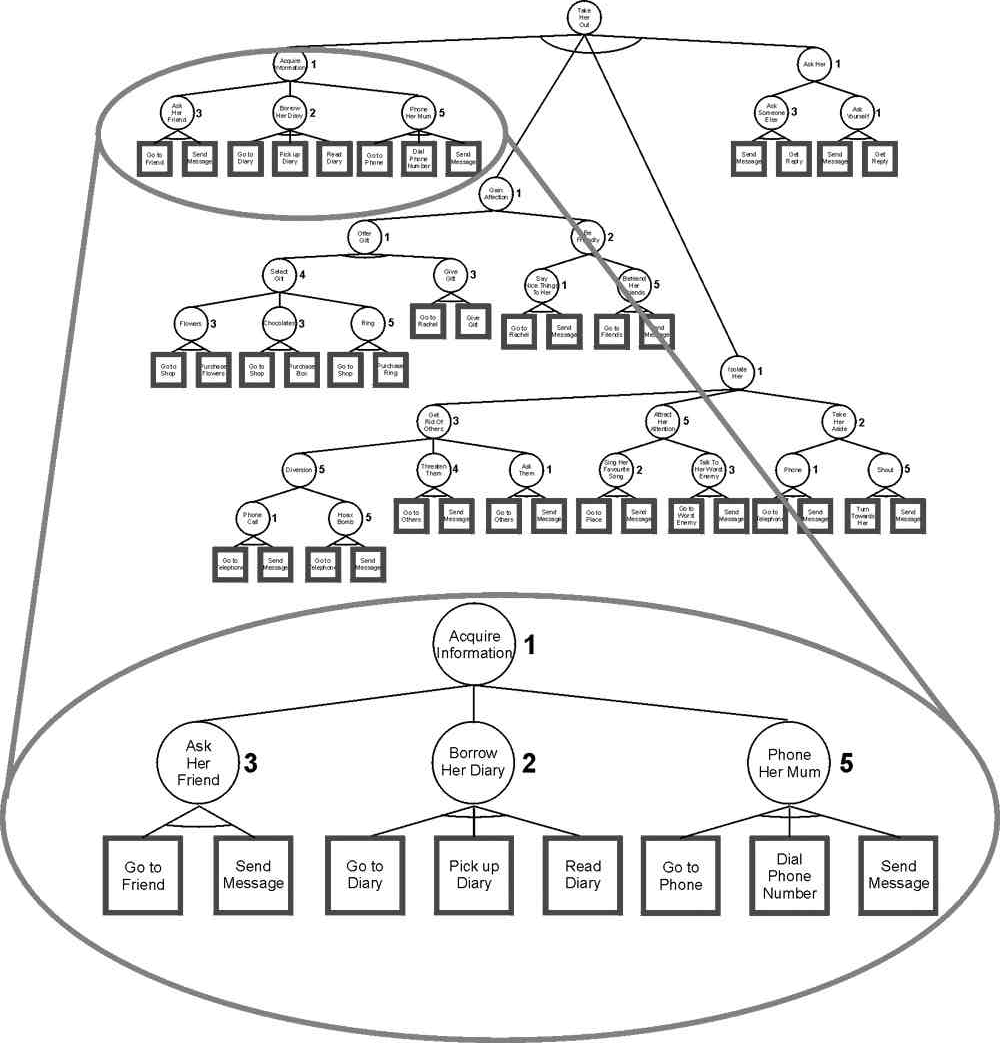
\includegraphics[scale=0.4]{images/htn.png}
  \caption{Hierarchical Task Networks}
  \label{fig:htn}
\end{figure}

La racine de cet arbre contient l'objectif principal du personnage. Les noeuds en dessous sont les différents sous-objectifs nécessaires à court terme pour réaliser l'objectif principal. Pour chaque sous-objectif, une liste d'actions possible à effectuer pour le réaliser donne au personnage différents moyens d'arriver à ses fins. Le choix dans ces actions s'effectue pour chaque sous-objectif en prenant les actions de gauche à droite, puis lorsque cette action est impossible, on prend la suivante. Un poids peut être associé à chacune de ces actions pour éviter un choix qui pourrait être mal perçu par les autres personnages par exemple.\\


\section{Modélisation de la personnalité}

Dans un jeu vidéo, beaucoup d'éléments peuvent être scriptés pour faire réagir les personnages d'une certaine façon. En revanche, en laissant le joueur assez libre dans ses actions, il faut trouver un autre moyen pour que les personnages non joueurs (PNJ) réagissent automatiquement, que ce soit par leurs actions directes, ou les émotions qu'ils laissent paraîtres.\\

\subsection{Relations sociales}

Comme présenté dans ~\cite{IRIS:conf/aiide/OchsSC2008}, la plupart des jeux de rôles ou des jeux d'aventures plongent le joueurs dans un rôle précis, avec un contexte déjà établie. L'impact des actions du joueurs sont alors généralement simplifiés a :

\begin{itemize}
\item un alignement : bien ou mal, loyal ou chaotic, pouvant limiter
  les actions possibles du joueur ou générer différentes réactions de
  la part des PNJs

\item une réputation, connu de tous les PNJs, qui peut modifier
  l'attitude des PNJs envers le joueur (par exemple, un joueur avec
  une mauvaise réputation pourra se faire attaquer dès qu'il croisera
  un garde).
\end{itemize}

~\\
Des résultats tirés d'études psychologique peuvent être utilisés afin de représenter plus précisément les relations sociales. Dans la plupart des travaux précédents, les chercheurs se sont basés sur un model static : la relation entre une émotion ressentie et la réaction d'un personnage était fixé. Nous allons voir ici un modèle de relations sociales dynamique, connecté à un modèle lié aux émotions : les émotions générées pendant une interaction peuvent produire différentes réactions, selon l'état du personnage et les émotions qu'il ressent.\\

Il n'existe pas de règles sur le nombre de variables nécessaires pour caractériser les relations sociales, mais on peut en ressortir 4 principales : 
\begin{itemize}
\item l'appréciation entre 2 personnages,
\item la dominance : la force qu'un personnage peut exercer sur un autre,
\item la solidarité : les ressemblances entre 2 personnages,
\item la familiarité, utile pour faire varier le type et le nombre d'informations partagées.
\end{itemize}
Il faut savoir que les relations sociales sont orientées et pas nécéssairement symétriques.\\

Pendant une interaction, les émotions ressenties par les 2 interlocuteurs peuvent changer leurs relations. En utilisant un modèle émotionnel, on représente l'état émotionnel par 4 vecteurs (sur [-1;1]) :
\begin{itemize}
\item joie / angoisse,
\item espoir / peur,
\item admiration / reproche,
\item fierté / honte.
\end{itemize}
Chacun des ces vecteurs vont agir positivement ou négativement sur les relations entre les personnages.

\subsection{Émotions}

Comme nous pouvons le voir dans ~\cite{IRIS:conf/aiide/Eladhari2010}, des recherches ont été faites afin de créer un prototype de monde de jeu multijoueur. Dans celui-ci, la personalité des personnages est la base de tout le fonctionnement. Chaque personnage possède des attributs de personnalité, et les joueurs voulant rejoindre doivent passer un test afin de déterminer leurs caractéristiques propres.\\

Pour faire ceci, ils utilisent un \rq{}Mind Module\lq{} (\textit{module d'esprit}), un agent semi-autonome représentant l'architecture de l'esprit des personnages. Il se base sur 4 types d'éléments : les traits, les émotions, les sentiments et l'humeur.\\
\begin{itemize}
\item Les traits représentent la personnalité de base d'un personnage, et avec une certaine relation avec les émotions, cela peut affecter la force avec laquelle un personnage va ressentir les évennements.
\item Les émotions représentent l'état d'esprit du personnage.
\item Les sentiments permettent de créer des liens entre les entités du monde. Cela peut agir sur les résultats d'un évennement par exemple.
\item L'humeur est séparée en 2 partie : l'humeur intérieure, c'est-à-dire la façon dont un personnage se sent, et extérieure, ce qu'il va montrer aux autres.
\end{itemize}
~\\
Ces éléments ne sont pas tous modifiés de la même façon. En effet, les traits sont fixés lors de la création du personnage et ne changeront pas. Les émotions ressenties vont diminuer rapidement après quelques minutes. À l'inverse, l'humeur peut rester pendant plusieurs heures.


\section{Conclusion}

Comme nous avons pu le voir, il existe différents moyens de représenter les comportements des personnages. L'utilisation des émotions semble cependant nécessaire pour permettre une réaction naturelles, en relation avec les évennements perçus par un personnage.



\bibliography{sources/bibliographieST}{}
\bibliographystyle{plain}
\end{document}
